% !TeX root = ../main.tex
% Add the above to each chapter to make compiling the PDF easier in some editors.

\chapter{Introduction}\label{chapter:introduction}
The rapid and continuous development of \ac{AI} has given birth to numerous
applications that have pushed the boundaries of what we previously believed to be possible.
This thesis will delve into one of the most fascinating and alarming developments in this
field, deepfakes. This document seeks to provide an exhaustive review of the current state
of the art in publicly-available deepfake detection tools.



\section{Background and Motivation}\label{chapter:backgroundAndMotivation}
In an era where digital media forms the cornerstone of communication, the advent of deepfakes,
\ac{AI}-enabled synthetic media, poses an unprecedented challenge to information integrity.
Deepfakes, a portmanteau of `deep learning' and `fake', is a technology that manipulates or
fabricates audio-visual content to make it appear real, often indistinguishable from the original.
An example of a generated and altered image can be seen in 

\begin{figure}[hb]
    \centering
    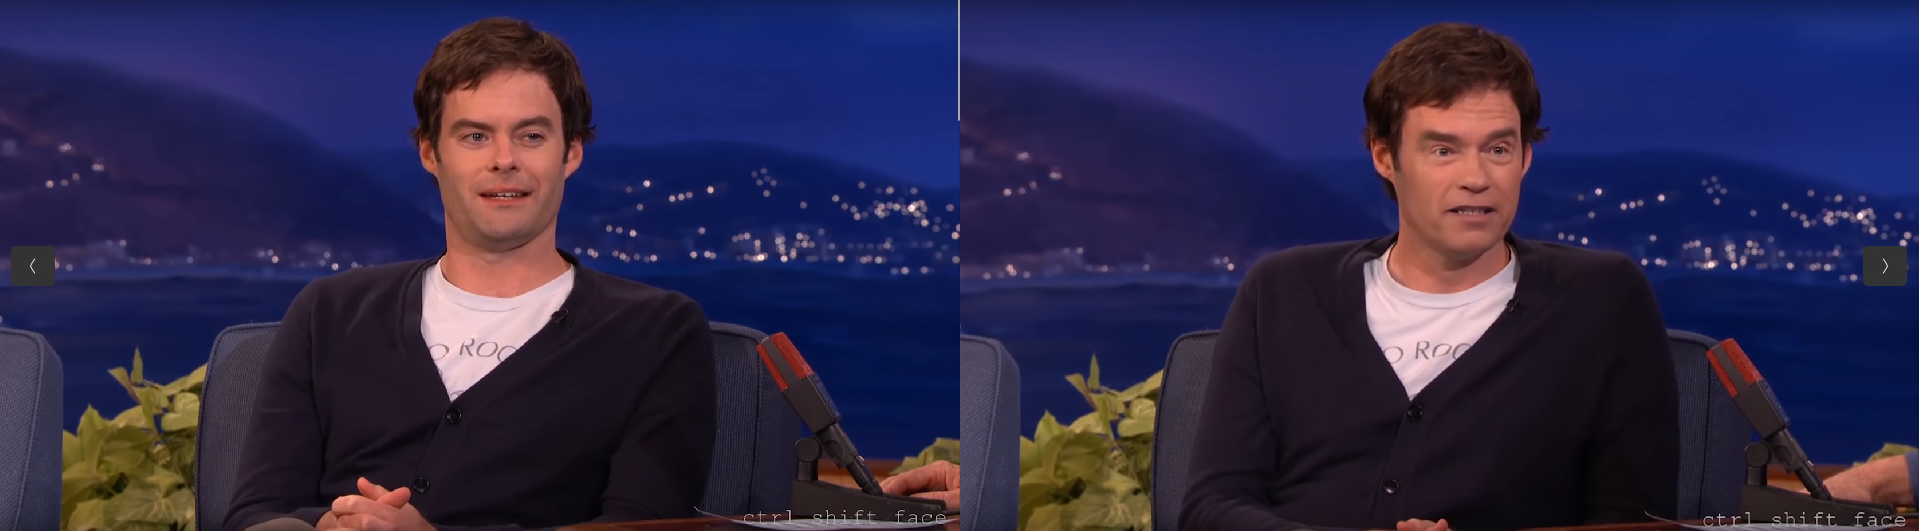
\includegraphics[scale=0.289]{figures/bill-arnold}
    \caption{Deepfake of Bill Hader impersonating Arnold Schwarzenegger. Screenshot from~\cite{bill-hader}}\label{fig:bill-hagel}
\end{figure}

The proliferation of deepfake technology become initially sparked with the aid of 
its software in creating misleading movie star images and videos, before quickly 
expanding into different sectors. One of the earliest examples that drew widespread 
interest to deepfakes was a video made by an anonymous Reddit user named `deepfakes' in late 2017.
This consumer started out to publish digitally altered pornographic motion pictures, 
realistically swapping the faces of actresses onto the bodies of porn stars. 
However, it wasn't lengthy earlier than the era was used out of doors of pornographic content.

An awesome instance that virtually established the electricity of deepfakes, 
and arguably delivered it to mainstream attention, turned into a video of former 
U.S. President Barack Obama, released in April 2018 by Buzzfeed and Jordan Peele~\cite{peele,10.1145/3371409}. 
The video features a deepfake of Obama announcing matters he by no means clearly 
stated, with Peele providing the voiceover. This deepfake video, considered by 
tens of millions, efficaciously highlighted the capability misuse of this generation 
in spreading misinformation and propaganda.

In recent years, the sophistication of deepfake technology has reached an unprecedented level. 
An interesting example of this progression can be seen in the creation of `Tom Cruise deepfakes' 
that circulated on social media in early 2021. The videos, created by Belgian visual effects 
artist Chris Ume in collaboration with actor Miles Fisher, who impersonated Cruise's voice 
and mannerisms, were shared on TikTok under the account name @deeptomcruise\footnote{\url{https://www.tiktok.com/@deeptomcruise}}. 
These deepfake videos show the synthetic `Tom Cruise' doing various activities --- performing 
a magic trick, playing golf, or simply telling a story about Mikhail Gorbachev~\cite{deeptomcruise}.

The `Tom Cruise deepfakes' took the internet by storm due to their uncanny resemblance to the 
real actor, in terms of both appearance and behavior. Unlike the early deepfake videos, which 
often exhibited glaring imperfections, these deepfakes were so convincing that many viewers 
initially believed they were watching the actual Tom Cruise. This level of realism underscored 
the strides made in deepfake technology, while simultaneously highlighting the potential 
dangers of its misuse.

Driven by advances in machine learning, especially deep learning, deepfake technology has
grown significantly in sophistication and accessibility. The potential applications of
deepfakes range from benign, such as in film production and entertainment, to malicious uses,
including disinformation campaigns, identity theft, and deepfake pornography. As these
applications become more widespread, deepfake technology has raised profound questions and
challenges for society, especially regarding media authenticity, privacy, and cybersecurity.

However, it is not just the creation of deepfakes that has improved; strides have also been made 
in detection. There are now more sophisticated, \ac{AI}-powered tools that can analyze videos 
and images for signs of manipulation. These tools operate on multiple levels, from detecting 
inconsistencies in lighting and shadows to looking for signs of digital artifacts and abnormal 
facial movements. But as detection tools become more sophisticated, so too do the techniques 
used to create deepfakes. This constantly evolving technological arms race underscores the 
critical need for ongoing research and development in deepfake detection.

In response to these challenges, there is an increasing need for robust and reliable
deepfake detection tools. However, despite the flurry of research and development in this
area, a comprehensive understanding and evaluation of the available detection tools remain
elusive. This knowledge gap not only impedes the technological advancements in deepfake
detection but also complicates the task of policy-making and regulation in this sphere.

This thesis is motivated by the need to bridge this gap and advance our understanding of
publicly-available deepfake detection tools. By examining these tools, this study aims to
contribute to the ongoing efforts to mitigate the risks associated with deepfakes and uphold
the integrity of digital media.


\section{Thesis Structure}\label{chapter:structure}
Understanding the structure of this thesis is essential for a comprehensive grasp of the 
research, as it follows a logical and systematic progression. It starts by laying the basic 
groundwork, then gradually delves deeper into the specifics of the study, eventually 
culminating in a synthesis of findings and forward-looking discussions. Below is a 
detailed outline of the thesis structure, which serves as a roadmap for navigating 
the document.

This initial section lays the foundation for the thesis. It provides an overview of deepfakes, 
introduces the topic of deepfake detection, and outlines the significance and timeliness 
of the study. It presents the objectives of the research, clearly stating what the study 
aims to achieve. The scope and limitations are also discussed here, delineating the 
boundaries of the research and acknowledging its constraints. The introduction serves 
as a guide, setting the reader's expectations for the rest of the thesis.

The literature review provides a comprehensive survey of the existing body of knowledge 
related to deepfakes and their detection. The section begins with the history of 
deepfakes, tracing their evolution over time. It then delves into the techniques used 
to create deepfakes, giving the reader an understanding of the technology behind them. 
This section also highlights the ethical and legal concerns surrounding deepfakes and 
the countermeasures and detection methods currently in place. By identifying gaps and 
shortcomings in the existing literature, this section also underscores the relevance 
and value of the present study.

Section three, the research design and methods adopted for the study are outlined. 
The section provides detailed information on how the publicly-available deepfake 
detection tools were selected for analysis. It also discusses the evaluation metrics 
used to test the effectiveness of these tools and the datasets used for testing. 
By detailing these elements, the section ensures that the research process is 
transparent and replicable.

Section four offers a comprehensive analysis of the selected deepfake detection tools. 
Each tool is explored in detail, discussing its working mechanisms, strengths, and 
potential limitations. This section also provides a comparative analysis of the tools, 
highlighting their relative strengths and weaknesses. Such a thorough examination is 
crucial to offer an in-depth understanding of the current landscape of publicly-available 
deepfake detection tools.

The fifth section takes the analysis from theory to practice, exploring real-world instances 
where deepfakes and their detection have played a significant role. The case studies 
are chosen to represent a variety of sectors and scenarios, thereby providing a broad 
view of the practical implications and challenges associated with deepfakes and their 
detection.

The sixth section presents the empirical findings from the evaluation of the selected tools. 
It provides a detailed report of how each tool performed across various tests, offering 
valuable insights into their effectiveness. This section serves as a vital point in the 
thesis, where collected data is introduced to support or challenge theoretical assertions.

The final section synthesizes the findings and discussions from the previous section and 
reflects on their contribution to the field. It provides a summary of the research, 
revisits the objectives, and discusses the extent to which they were achieved. It also 
identifies potential directions for future research, offering suggestions for how the 
field can continue to evolve and adapt in response to the dynamic nature of deepfakes.

In sum, the thesis follows a clear and logical structure that mirrors the research 
process, moving from the contextualization of the problem, through detailed analysis 
and evaluation, to the synthesis of findings and concluding reflections. This structure 
enables a thorough, systematic exploration of the state of the art of publicly-available 
deepfake detection tools, ensuring that the study is both comprehensive and focused.


\section{Objectives of the Study}\label{chapter:objectives}
The primary objective of this thesis is to provide a comprehensive and in-depth exploration 
of the state of the art in publicly-available deepfake detection tools. This ambitious aim 
necessitates a multi-pronged approach, encompassing a wide array of secondary objectives 
that collectively serve to create a well-rounded examination of the topic. The identification 
and elaboration of these objectives provide a roadmap for the study, with each one serving 
as a crucial stepping-stone toward the main goal.

The first objective is to trace the development of deepfake technology from its roots to its 
current state. This involves an in-depth exploration of the early techniques used in deepfake 
generation, the seminal developments that spurred its evolution, and the resulting modern 
methods capable of producing incredibly realistic and convincing deepfakes. Understanding the 
sophistication of the technology that we're attempting to counter is crucial, and can provide 
vital context for the subsequent investigation of detection tools.

While closely related to the first objective, the second objective delves deeper into the 
technical aspects of deepfake generation. The objective is to dissect and comprehend the 
underlying algorithms, techniques, and processes involved in creating deepfakes. This involves 
exploring machine learning and deep learning methods, such as autoencoders and 
\ac{GAN}s, that are fundamental to deepfake technology. This deep understanding can 
then be leveraged to better comprehend the mechanisms of deepfake detection tools.

At the heart of this thesis lies the primary investigative objective: the identification 
and detailed exploration of existing, publicly-available deepfake detection tools. 
This involves a comprehensive audit of these tools, an examination of their origins, 
the technology they employ, and their evolution in response to ever-improving deepfake 
generation techniques. This objective is crucial, as it provides the groundwork for 
the evaluation stage, providing us with a detailed understanding of what we're 
evaluating and why.

Having laid a thorough foundation with the previous objectives, the next goal is to objectively 
evaluate the performance of the identified deepfake detection tools. This assessment 
will be conducted using a wide array of deepfakes, evaluating the effectiveness, 
accuracy, and reliability of each tool across a spectrum of test cases. This rigorous 
evaluation process aims to determine how these tools fare against various types of 
deepfakes, offering insights into their strengths, weaknesses, and areas for potential 
improvement.

Given the potential for deepfakes to have significant societal impacts, a key objective of this 
study is to delve into the ethical, legal, and societal implications surrounding deepfakes 
and their detection. This includes exploring the potential risks deepfakes pose to 
information authenticity and privacy, as well as the ethical quandaries arising from 
the use of AI in deepfake detection. By illuminating these broader implications, the 
study aims to offer a more holistic view of the deepfake landscape.

The final objective of this study is to use the findings to propose concrete, actionable 
recommendations for future development in deepfake detection. These could range from 
technical enhancements for existing tools, the development of new, innovative detection 
methodologies, or even policy recommendations aimed at governing the use and detection 
of deepfakes. By offering well-founded recommendations, this study aims to play a part 
in shaping the future direction of deepfake detection.

Collectively, these objectives provide a comprehensive framework for the study, allowing 
for a various exploration of the world of deepfakes and their detection. Each 
objective is not an end in itself but serves as a stepping stone towards the overall 
goal: to deepen our understanding of the state of the art in publicly-available deepfake 
detection tools and to contribute meaningfully to the ongoing efforts to mitigate the 
risks posed by deepfakes.

\section{Scope and Limitations}\label{chapter:scope}
The study of deepfakes and their detection is a broad field, involving a range of complex and 
interrelated topics. Therefore, it is essential to define the specific scope and 
limitations of this thesis to clarify what it will and will not cover. These boundaries 
not only provide clarity but also help ensure that the research is feasible and can delve 
into the chosen topics in sufficient depth.

\subsection{Scope of the Study}
The primary focus of this thesis is on the analysis and evaluation of publicly available 
deepfake detection tools. It will cover both the technical and societal aspects of these 
tools, including their performance, methodologies, implications, and potential areas for 
future development. It will also provide an overview of the current state of deepfake 
technology, from its historical development to its modern techniques and applications.

The thesis will mainly concentrate on visual deepfakes, encompassing both images and 
videos, aiming to offer a thorough understanding of the deepfake environment. The 
research will also explore the dual nature of deepfakes, examining their harmless 
and harmful applications. This exploration is crucial to fully comprehend the 
difficulties involved in detecting deepfakes.

\subsection{Limitations of the Study}
Despite its broad scope, the study is subject to several limitations that should be 
acknowledged. Firstly, due to the rapid pace of technological advancements in the field 
of deep learning and \ac{AI}, the state of the art in deepfake technology and detection tools 
can change swiftly. As a result, while the thesis aims to provide an up-to-date overview 
of the field, some of the information might become outdated shortly after publication.

Secondly, given the focus on publicly-available tools, this thesis might not capture 
the full spectrum of deepfake detection methodologies. Many sophisticated tools and 
techniques might be proprietary or classified information, not accessible for public 
use or scrutiny. Thus, while this study will provide a comprehensive overview of the 
available tools, it might not cover the absolute cutting edge in deepfake detection.

Thirdly, while the study aims to objectively evaluate the performance of deepfake 
detection tools, it's important to note that this evaluation is based on the 
available datasets and metrics. Variations in these datasets, such as the quality 
and diversity of the deepfakes included, can impact the results. Moreover, no 
single evaluation metric or dataset can fully capture the effectiveness of a tool 
in all real-world scenarios.

Fourthly, while the study will explore the societal, ethical, and legal implications 
of deepfakes and their detection, a comprehensive analysis of these complex and 
evolving issues is beyond its scope. These aspects will be discussed primarily in 
relation to the main focus of the thesis --- deepfake detection tools --- and may not 
cover all the potential implications of deepfakes.

Finally, the study is limited by the inherent challenges associated with deepfake 
detection. Deepfakes are a result of advanced \ac{AI} and machine learning techniques, 
and detecting them is a complex task that is still an area of active research. 
Therefore, the study's findings should be viewed in light of these inherent difficulties.

\subsection{Delimitations of the Study}
While limitations are factors that are out of the researcher's control, delimitations 
are boundaries set by the researcher. In this study, due to time and resource constraints, 
the analysis will be limited to a representative sample of publicly-available deepfake 
detection tools, rather than an exhaustive list of all available tools. Similarly, while 
the study will discuss a few illustrative examples of deepfake applications and case 
studies, it will not provide a comprehensive review of all possible uses or instances 
of deepfakes.

By acknowledging these scope, limitations, and delimitations, this thesis aims to 
provide a focused, in-depth, and accurate exploration of publicly-available deepfake 
detection tools while being transparent about its boundaries and potential areas of 
uncertainty.
